\documentclass[border=7pt]{standalone}
\usepackage{tikz}
\begin{document}
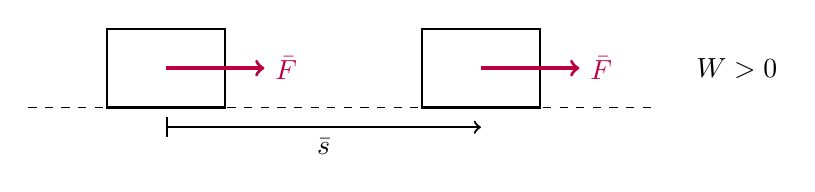
\begin{tikzpicture}
  % gólf
  \draw [dashed](0,0) -- (8,0);
  % kassi
  \draw [thick] (1,0) rectangle (2.5,1);
  \draw [thick] (6.5,0) rectangle (5,1);


  % kraftar
  \draw [very thick, ->, purple] (1.75,0.5) -- (3,0.5) node [right] {$\bar{F}$};
  \draw [very thick, ->, purple] (5.75,0.5) -- (7,0.5) node [right] {$\bar{F}$};
  \node (c) at (9,0.5) {$W > 0$};
  \draw [thick, |->] (1.75, -0.25) --(5.75, -0.25);
  \node (c) at (3.75, -0.5) {$\bar{s}$};
\end{tikzpicture}
\end{document}
